\documentclass{article}
\usepackage{pythonhighlight}
\usepackage{graphicx}
\usepackage{subfigure}
\usepackage{ctex}
\usepackage[left=3cm,top=3cm,right=3cm]{geometry}
\usepackage{hyperref}
% TITLE PAGE CONTENT %%%%%%%%%%%%%%%%%%%%%%%%
%%%%%%%%%%%%%%%%%%%%%%%%%%%%%%%%%%%%%%%%%%%%%
\newcommand{\labno}{13}
\newcommand{\labtitle}{EE208 PyTorch}
\newcommand{\authorname}{周李韬}
\newcommand{\studentno}{518030910407}
\newcommand{\classno}{F1803016}
% END TITLE PAGE CONTENT %%%%%%%%%%%%%%%%%%%%


\begin{document}

\begin{center}
{\LARGE \textsc{Laboratory No. \labno:} \\ \vspace{4pt}}
{\Large \textsc{\labtitle} \\ \vspace{4pt}} 
\rule[13pt]{\textwidth}{1pt} \\ \vspace{15pt}
{\large By: \authorname \\ \vspace{10pt}
No. \studentno \\ \vspace{10pt}
SJTU \classno \\ \vspace{10pt}
\today \vspace{20pt}}
\end{center}



\section{实验准备}

\subsection{实验环境}
\begin{itemize}
\item\textbf{Environment} Python 3.7
\item\textbf{Packages} PyTorch 1.3.1, matplotlib
\item\textbf{Tools} Pycharm 2018.2 on Windows 10
\end{itemize}

\subsection{实验目的}

本实验中,我们需要利用PyTorch训练模型,实现初等函数的拟合和CIFAR-10进行图片分类。

\subsection{实验原理}
机器学习的目的和核心是寻找一个函数,经典的神经网络中包括输入层、输出层和中间层(隐藏层),在一层神经网络中,通过对输入的边权值做加权求和,经过一次非线性函数的映射后即可得到输出层。这一层的输出又可以作为下一层的输入,从而叠加形成许多隐藏层,形成神经网络。现代神经网络的层数非常多(可能有50层甚至几百层),对这种多层神经网络的训练,可以认为就是深度学习。本实验中,我们通过PyTorch进行深度学习的训练,实现初等函数的拟合和图片分类。


\section{实验过程}

\subsection{初等线性函数的拟合}

在PyTorch中已经内置好了相关的神经网络模型,训练原理如下。

\begin{python}
1. 随机读入一个batch的数据(x, target_y)。[len(x)=len(target_y)=batch size, 即x[i]对应target_y[i]
2. 把x输入模型,得到predicted_y[predicted_y=model(x)]
3. 比较predic_y和target_y, 计算误差(mse)
4. 根据误差,告知模型各参数的修正趋势(各参数是该变大还是减小)[loss.backward()],并依据此趋势更新参数[optimizer.step()]
5. 回到1
\end{python}

我们在拟合函数的实验中只需要调整两个参数,即Epoch\_Num(训练轮次数)和learning\_rate(修正幅度)。我们首先对函数

$$ f(x) = x^2 + 2\sin{x}+\cos{x-1}-5, x \in \left[-5,5\right]$$

进行拟合。实验结果如下所示。

\subsubsection{更改NUM\_TRAIN\_EPOCHS}


\begin{figure}[htb]
\centering
\subfigure[EPOCH = 100, LearningRate = 0.01]{
\begin{minipage}[htb]{6cm}
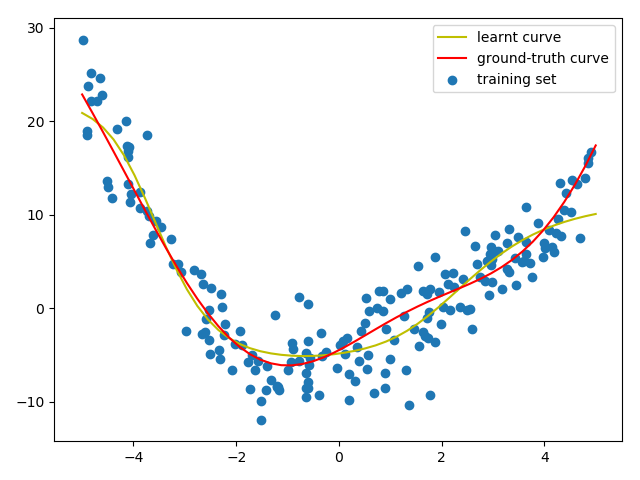
\includegraphics[width=6cm]{img/plot100_01.png}
%\caption{EPOCH = 100, LearningRate = 0.01}
\end{minipage}%
}%
\subfigure[EPOCH = 1000, LearningRate = 0.01]{
\begin{minipage}[htb]{6cm}
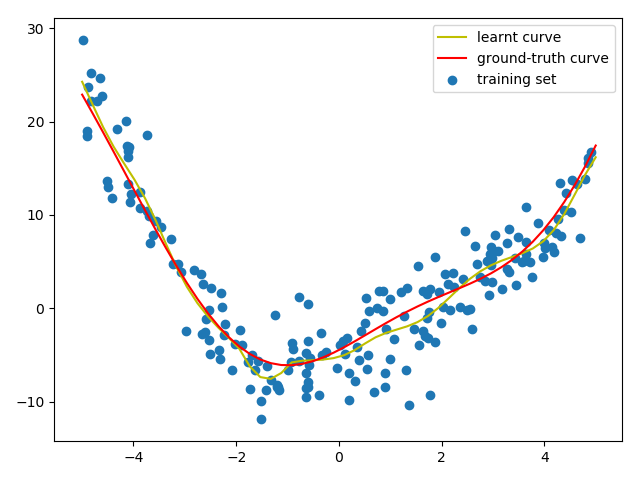
\includegraphics[width=6cm]{img/plot1000_01.png}
%\caption{EPOCH = 1000, LearningRate = 0.01}
\end{minipage}%
}%

\subfigure[EPOCH = 10000, LearningRate = 0.01]{
\begin{minipage}[htb]{6cm}
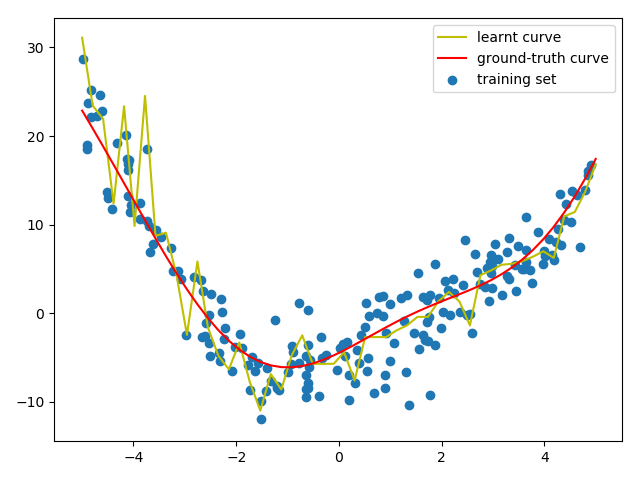
\includegraphics[width=6cm]{img/plot10000_01.png}
%\caption{EPOCH = 10000, LearningRate = 0.01}
\end{minipage}%
}%
\subfigure[EPOCH = 50000, LearningRate = 0.01]{
\begin{minipage}[htb]{6cm}
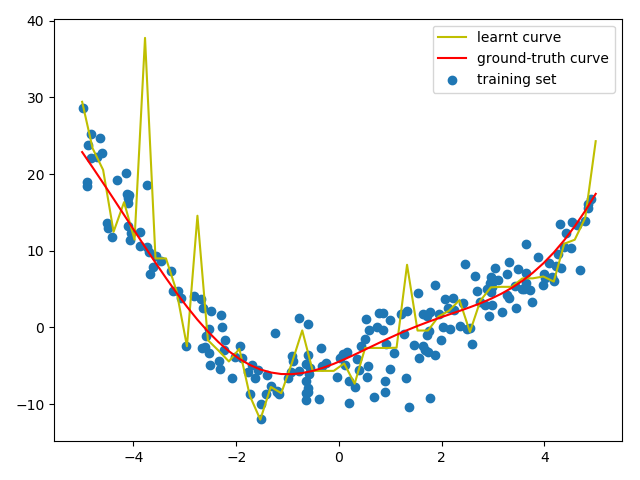
\includegraphics[width=6cm]{img/plot50000_01.png}
%\caption{EPOCH = 50000, LearningRate = 0.01}
\end{minipage}%
}%
\centering
\caption{实验A部分结果}
\label{fig:funA}
\end{figure}

训练结果如图\ref{fig:funA}所示。从实验中可知,EPOCH越高,LOSS越小,这是因为我们训练拟合函数的方法朝着LOSS减小的方向调整参数的。在EPOCH次数不是很大的情况下,训练次数越多,拟合曲线与原曲线的相似程度越大。但若EPOCH过大,在我们训练集取点较稀疏的地方,会出现明显的峰值,出现过拟合的现象,如图d所示。此外,我们也注意到,在训练轮次达到50000次的情况下,LOSS已不能再下降了,甚至有时会出现上下浮动的情况,表明进一步的训练已经对提升模型的精确程度无效了。


\subsubsection{更改LEARNING\_RATE}

训练结果如图\ref{fig:funB}所示。Learning Rate是我们每次训练对模型调整的参数大小,learning rate决定了权值更新的速度。固定训练轮次不变,改变learning rate,总体而言,learning rate越高,曲线越平滑。从拟合效果方面看,在图a中,learning rate过大使结果会在目标周围浮动过大,在图c中,learning rate过小会使拟合速度过慢,在训练1000轮后拟合曲线两端与原曲线有较大偏离。因此learning rate与拟合效果密切相关,理想的learning rate应该随训练轮次数依次降低,从而更有效地趋近训练目标。

\begin{figure}[htb]
\centering
\subfigure[EPOCH = 1000, LearningRate = 0.1]{
\begin{minipage}[htb]{6cm}
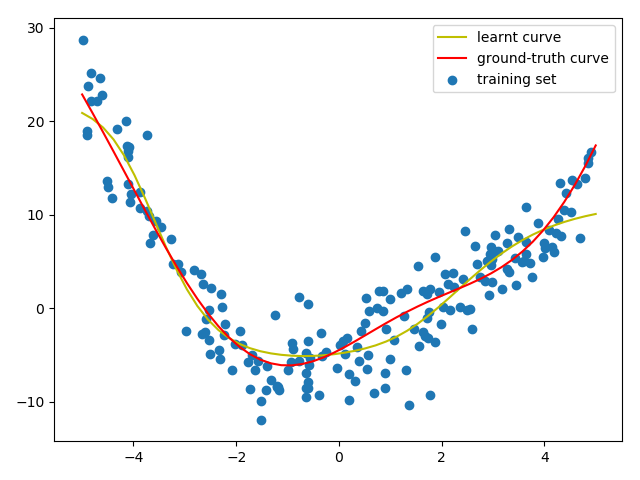
\includegraphics[width=6cm]{img/plot100_01.png}
\end{minipage}%
}%
\subfigure[EPOCH = 1000, LearningRate = 0.01]{
\begin{minipage}[htb]{6cm}
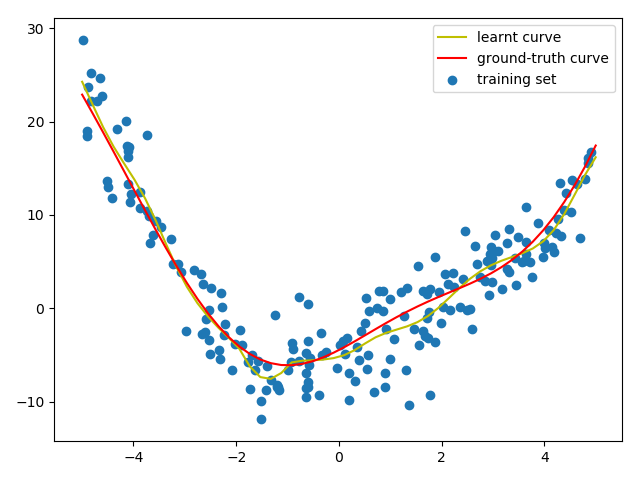
\includegraphics[width=6cm]{img/plot1000_01.png}
\end{minipage}%
}%

\subfigure[EPOCH = 1000, LearningRate = 0.001]{
\begin{minipage}[htb]{6cm}
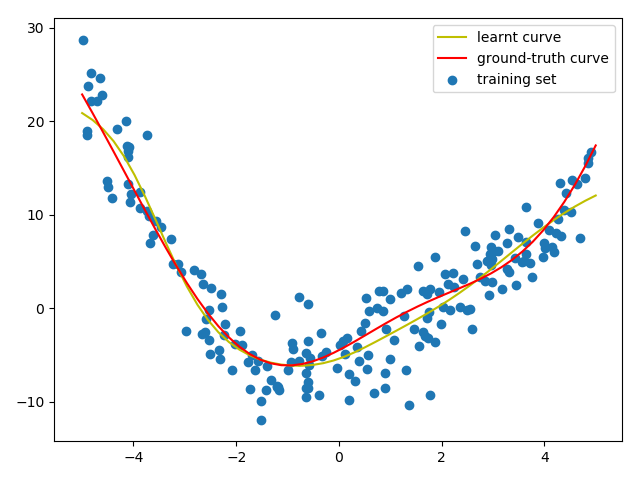
\includegraphics[width=6cm]{img/plot1000_001.png}
\end{minipage}%
}%
\centering
\caption{实验B部分结果}
\label{fig:funB}
\end{figure}

要取得较好的拟合效果,我们需要兼顾训练轮次和学习率的关系,学习率低意味着训练轮次要高才能达到较好的拟合,但也要注意不能训练过多轮导致过拟合,经过调试,我们在$EPOCH = 2000, LR = 0.002$时取得了原函数较好的拟合,如图\ref{fig:funB2}所示。

\begin{figure}[htb]
\centering
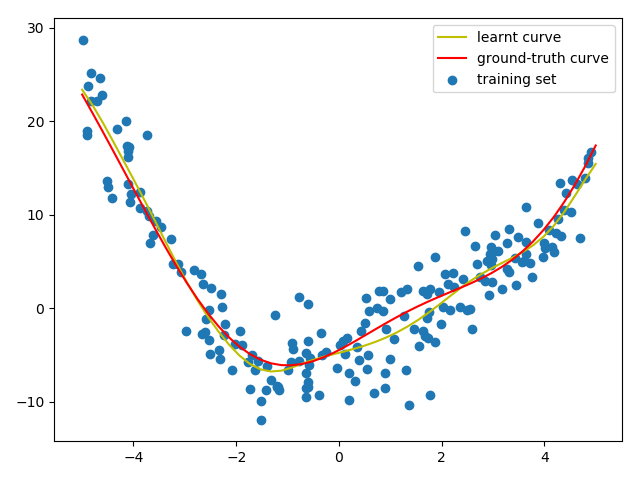
\includegraphics[width=13.5cm]{img/plot2000_002.png}
\caption{EPOCH = 2000, Learning\_Rate=0.002}
\label{fig:funB2}
\end{figure}


\subsubsection{自定义函数拟合}

由于本实验采用的模型是以多项式的方式在小区间内进行训练拟合的,因此对于局部变化率较小的函数,如指对函数、简单多项式函数,通过简单的调参,可以做到效果较好的拟合,如图\ref{fig:funC1}所示。

\begin{figure}[htb]
\centering
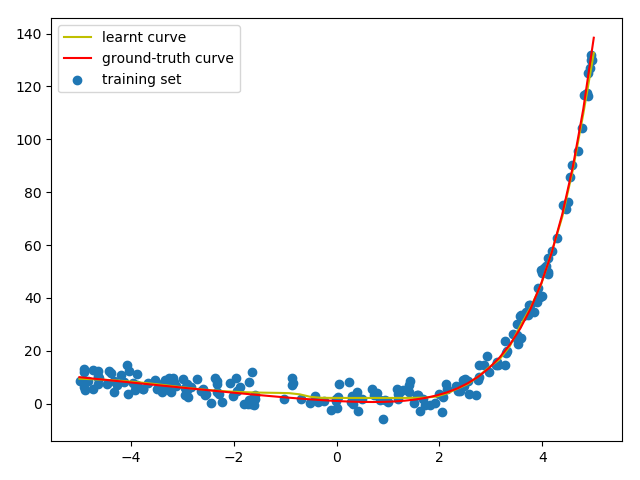
\includegraphics[width=13.5cm]{img/good.png}
\caption{对函数$f(x)=e^x - 2x$的拟合结果,EPOCH = 1500, Learning\_Rate=0.02}
\label{fig:funC1}
\end{figure}

\begin{figure}[htb]
\centering
\subfigure[EPOCH = 1000, LearningRate = 0.01]{
\begin{minipage}[htb]{6cm}
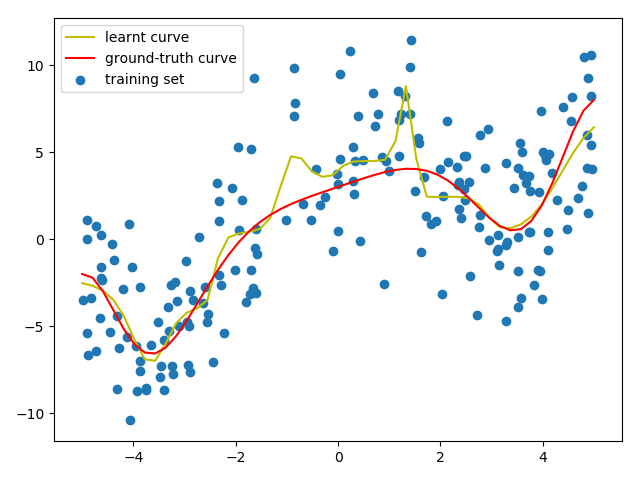
\includegraphics[width=6cm]{img/t1000_01.png}
\end{minipage}%
}%

\subfigure[EPOCH = 1000, LearningRate = 0.001]{
\begin{minipage}[htb]{6cm}
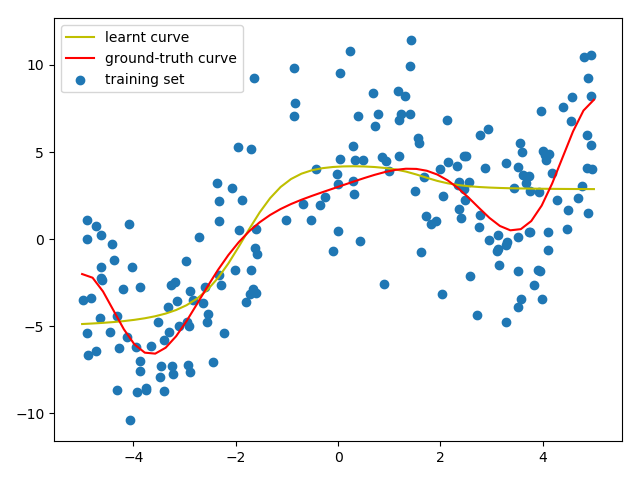
\includegraphics[width=6cm]{img/t1000_001.png}
\end{minipage}%
}%

\subfigure[EPOCH = 800, LearningRate = 0.01]{
\begin{minipage}[htb]{6cm}
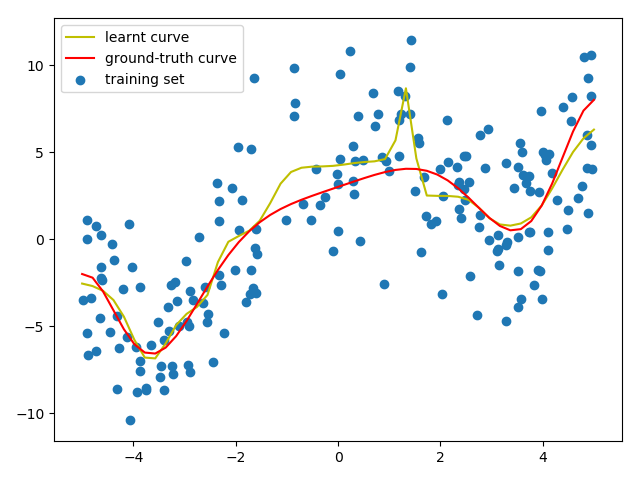
\includegraphics[width=6cm]{img/t800_01.png}
\end{minipage}%
}%
\subfigure[EPOCH = 1000, LearningRate = 0.006]{
\begin{minipage}[htb]{6cm}
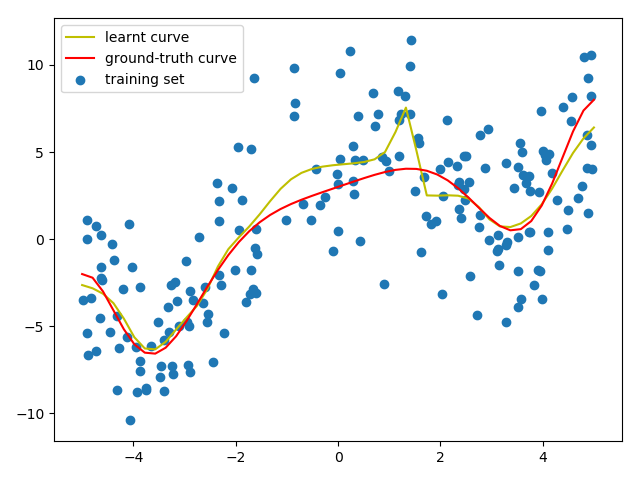
\includegraphics[width=6cm]{img/t1000_006.png}
\end{minipage}%
}%
\centering
\caption{实验C部分结果}
\label{fig:funC2}
\end{figure}

为了更好地观察训练轮次和学习率对函数拟合的影响,本实验选取了一个较为复杂的函数 $$ f(x) = 3 \cos{\frac{x^2}{4}} +  x $$ 该函数在$[-5,5]$区间内有若干极值点,我们的参数调整过程如图\ref{fig:funC2}。我们首先



\subsubsection{实验过程}

\section{实验总结}
\paragraph{概述}
本实验中,我们通过OpenCV实现了图像边缘检测的SIFT算法特征点的匹配与图像匹配度的计算。

\paragraph{感想}
通过本次实验的学习,我通过手动实现SIFT算法的图像预处理、梯度计算、特征点提取、特征向量计算等过程,对图像处理中的特征提取方法和思想有了更深的理解,也掌握了更多OpenCV和numpy矩阵操作的技巧。

\paragraph{问题}
本次实验中遇到的问题为匹配度不高。由于实验方法本身的精度限制,如我们在提取Harris角点时没有进行尺度空间的差分,从而难以得到真正意义上准确的特征角点,如我们在计算梯度时采用的是微分算子,没有达到SIFT要求的精确度,因此即便经过反复修改代码和调试参数后,我们也没有得到显著可观的匹配度提高。但我依然在调试的过程中,对SIFT算法的思想和原理有了更深的认识。

\paragraph{创新}
本实验中采用了Prewitt算子计算梯度,相较材料中给出的梯度计算方法有一定的提升。此外,代码中也灵活运用了filter2D、math.atan2等函数,简化了代码,提高了可读性。本实验还将SIFT计算封装为一个类对象,提高了可用性。

\end{document}

